\documentclass[pdflatex,compress,mathserif]{beamer}

%\usetheme[dark,framenumber,totalframenumber]{ElektroITK}
\usetheme[darktitle,framenumber,totalframenumber]{ElektroITK}

\usepackage[utf8]{inputenc}
\usepackage[T1]{fontenc}
\usepackage{lmodern}
\usepackage[bahasai]{babel}
\usepackage{amsmath}
\usepackage{amsfonts}
\usepackage{amssymb}
\usepackage{graphicx}
\usepackage{multicol}
\usepackage{lipsum}
\usefonttheme[onlymath]{serif}

\newcommand*{\Scale}[2][4]{\scalebox{#1}{$#2$}}%

\setbeamertemplate{caption}[numbered]

\title{MATEMATIKA DASAR}
\subtitle{Trigonometri}

\author{Mifta Nur Farid}

\begin{document}

\maketitle

\section{Pengukuran Sudut}

\begin{frame}
	\frametitle{Pengukuran Sudut}
	\begin{center}
		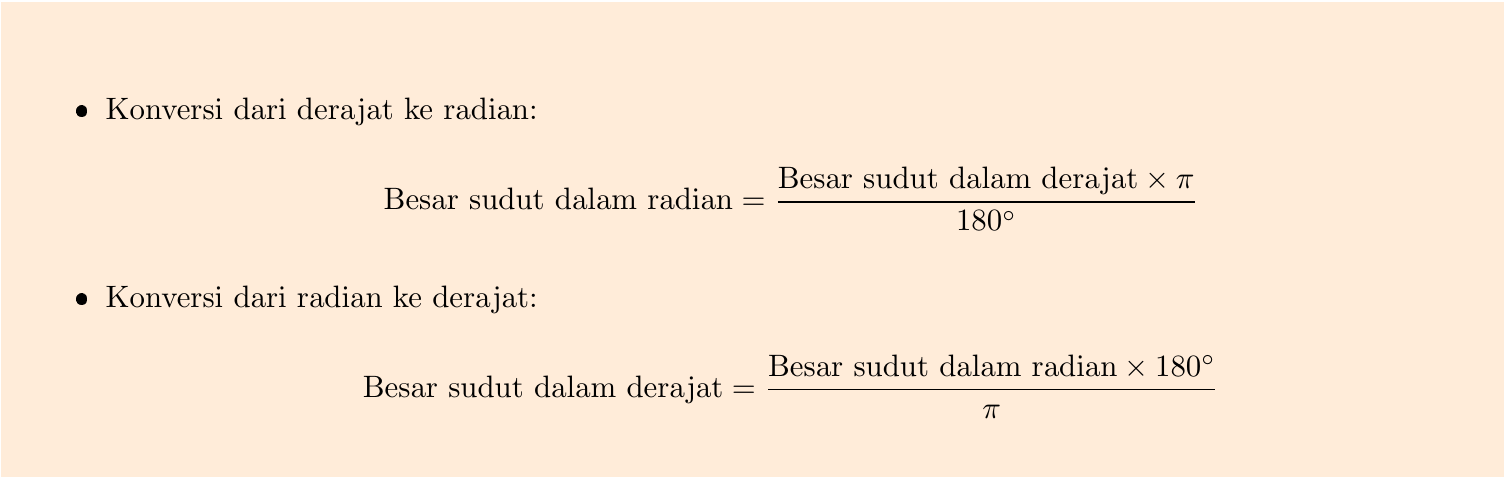
\includegraphics[width=\linewidth]{img/img01}
	\end{center}
\end{frame}

\begin{frame}
	\frametitle{Pengukuran Sudut}
	\begin{center}
		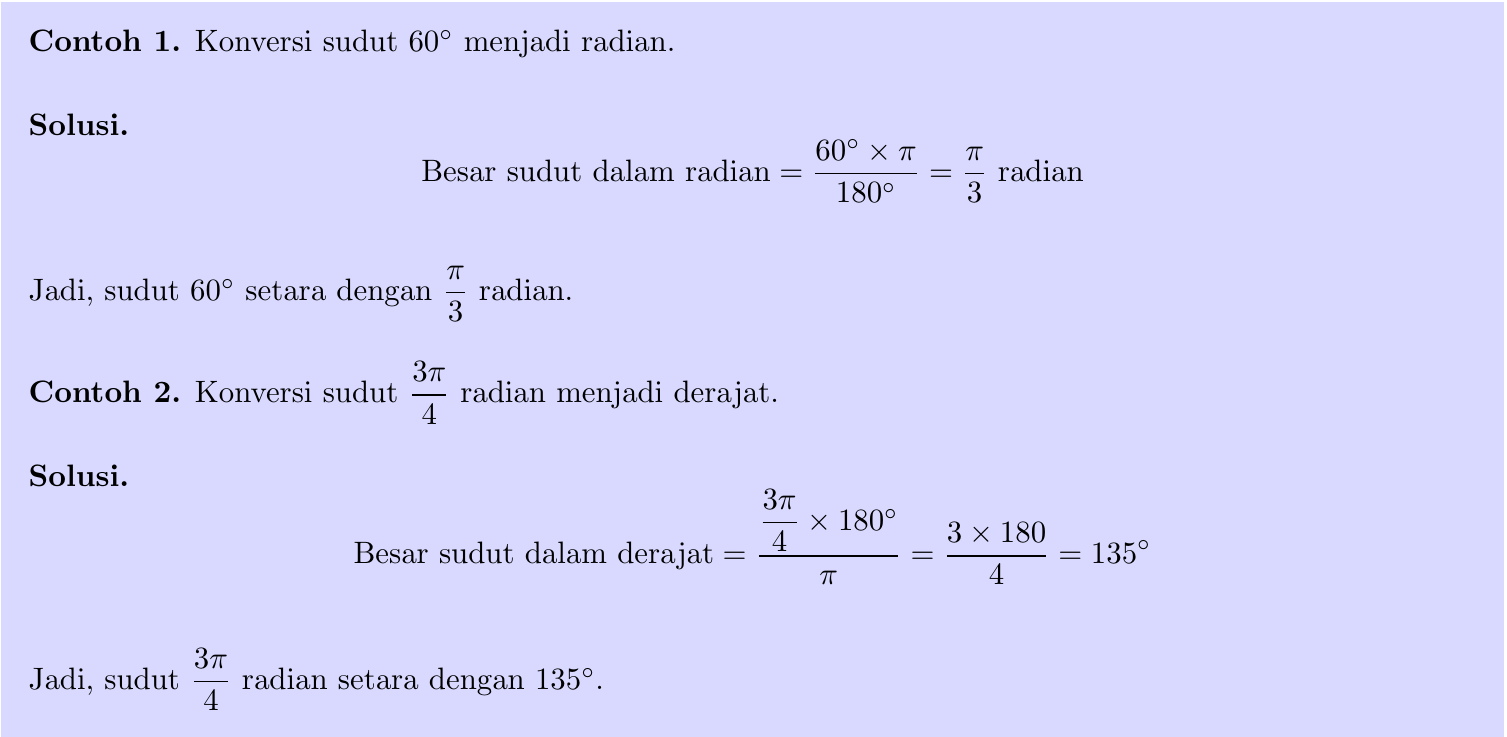
\includegraphics[width=\linewidth]{img/img02}
	\end{center}
\end{frame}

\section{Trigonometri Segitiga Siku-Siku}

\begin{frame}
	\frametitle{Trigonometri Segitiga Siku-Siku}
	\begin{center}
		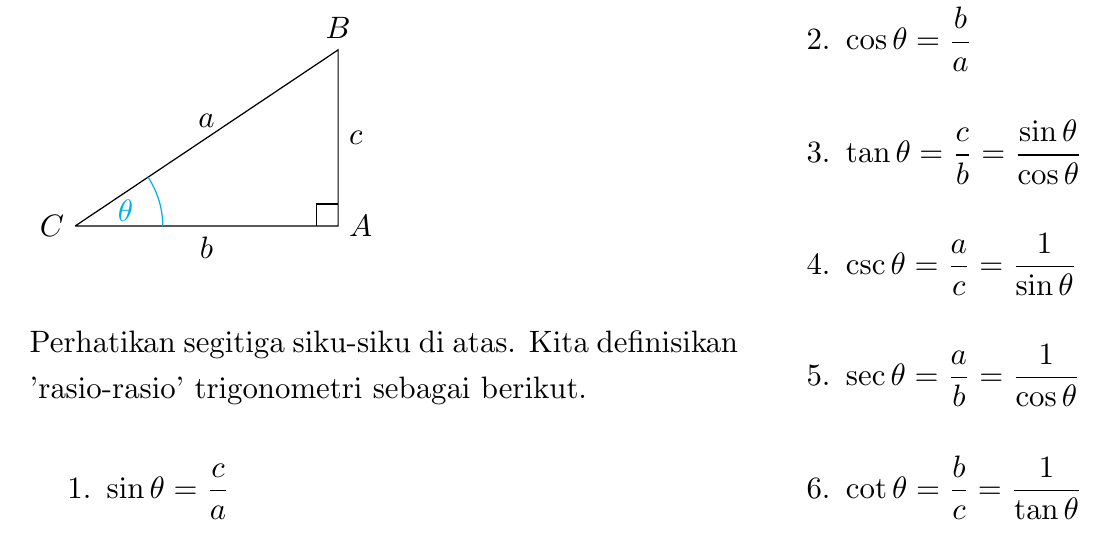
\includegraphics[width=\linewidth]{img/img03}
	\end{center}
\end{frame}

\begin{frame}
	\frametitle{Trigonometri Segitiga Siku-Siku}
	\begin{center}
		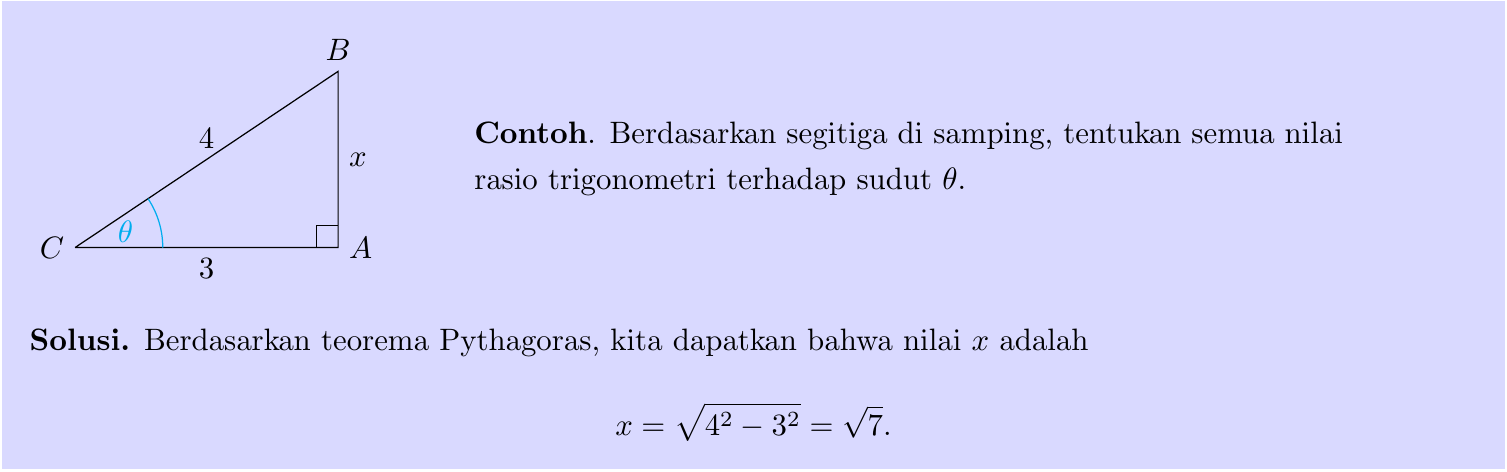
\includegraphics[width=\linewidth]{img/img04}
		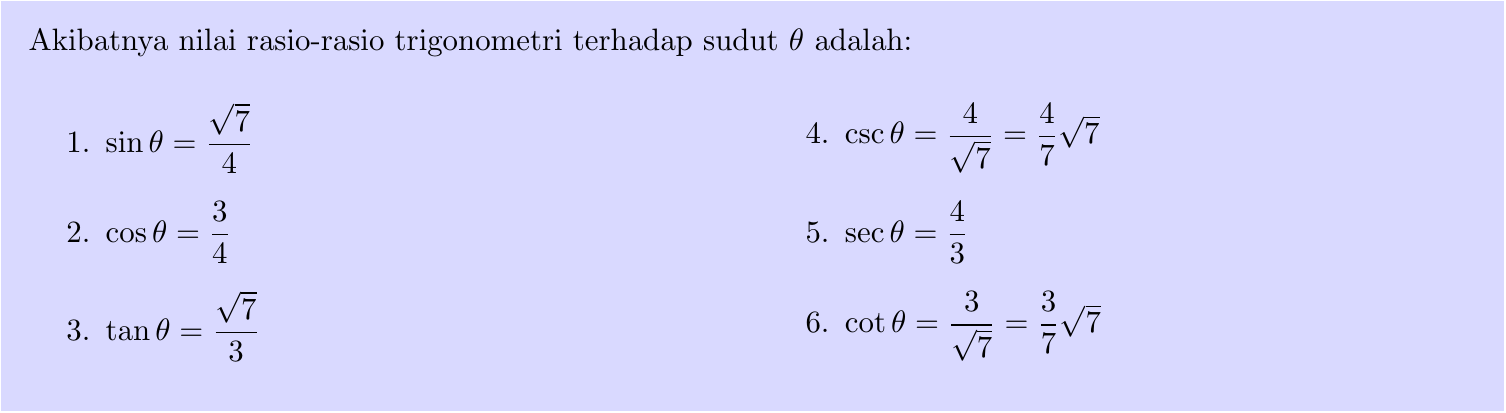
\includegraphics[width=\linewidth]{img/img05}
	\end{center}
\end{frame}

\section{Trigonometri Sebagai Fungsi}

\begin{frame}
	\frametitle{Trigonometri Segitiga Siku-Siku}
	\begin{center}
		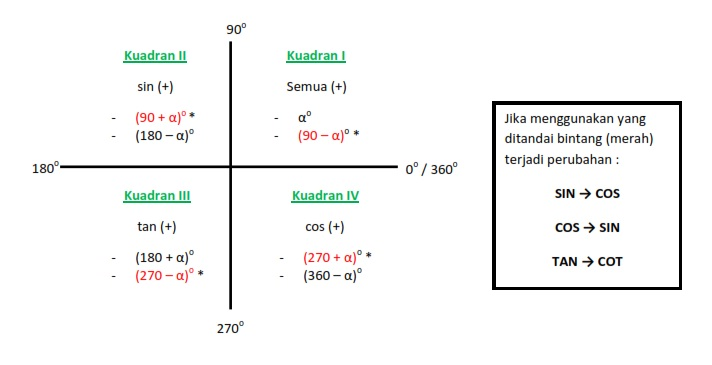
\includegraphics[width=\linewidth]{img/img06}
	\end{center}
\end{frame}

\section{Identitas Trigonometri}

\section{Persamaan Trigonometri}

\section{Aturan Sinus dan Cosinus}

\end{document}
